% Guida rapida di IPTV, edizione italiana. Compilare in questa cartella con:
%   pdflatex IPTV-Quick-Start-it.tex   (due volte, per l'indice)
\newcommand{\GuideLang}{italian}
\newcommand{\GuideTitle}{Guida rapida}
\newcommand{\TipLabel}{Suggerimento.}
% Shared layout of the IPTV quick start guides (one file per language:
% IPTV-Quick-Start.tex, IPTV-Quick-Start-it.tex, ...). Each sets, before
% % Shared layout of the IPTV quick start guides (one file per language:
% IPTV-Quick-Start.tex, IPTV-Quick-Start-it.tex, ...). Each sets, before
% % Shared layout of the IPTV quick start guides (one file per language:
% IPTV-Quick-Start.tex, IPTV-Quick-Start-it.tex, ...). Each sets, before
% \input{preamble}:
%   \GuideLang   babel language (english, italian, spanish, french, ngerman, portuguese)
%   \GuideTitle  the guide's title, used on the cover, in headers and the PDF
%   \TipLabel    the word that starts a tip box ("Tip.")
% Build any of them with pdflatex, twice (for the table of contents).
\documentclass[11pt,a4paper]{article}

\usepackage[T1]{fontenc}
\usepackage[utf8]{inputenc}
% shorthands=off: no language-specific active characters (they would clash
% with tables and addresses); only hyphenation and "Contents" etc. change.
\usepackage[shorthands=off,\GuideLang]{babel}
\usepackage{lmodern}
\usepackage[scaled=0.92]{helvet}
\renewcommand{\familydefault}{\sfdefault}
\usepackage[margin=2.2cm,headheight=14pt]{geometry}
\usepackage{graphicx}
\usepackage[table]{xcolor}
\usepackage{booktabs}
\usepackage{tabularx}
\usepackage{xltabular}
\usepackage{enumitem}
\usepackage{titlesec}
\usepackage{fancyhdr}
\usepackage{pifont}
\usepackage{amssymb}
\usepackage[hidelinks]{hyperref}

\newcommand{\version}{0.12}
\definecolor{accent}{HTML}{1E6FD9}
\definecolor{dim}{HTML}{5F6673}
\definecolor{notebg}{HTML}{EEF4FC}
\definecolor{warnbg}{HTML}{FFF6E0}
\definecolor{tvred}{HTML}{D32F2F}
\definecolor{tvgreen}{HTML}{2E7D32}
\definecolor{tvyellow}{HTML}{C9A400}
\definecolor{tvblue}{HTML}{1565C0}

\hypersetup{pdftitle={IPTV -- \GuideTitle}, pdfauthor={IPTV project}}
\setlist{itemsep=2pt, topsep=4pt}
\setlength{\parindent}{0pt}
\setlength{\parskip}{6pt}
\renewcommand{\arraystretch}{1.25}

\titleformat{\section}{\Large\bfseries\color{accent}}{\thesection}{0.6em}{}
\titleformat{\subsection}{\large\bfseries}{\thesubsection}{0.6em}{}
\titlespacing*{\section}{0pt}{14pt}{6pt}
\titlespacing*{\subsection}{0pt}{10pt}{4pt}

\pagestyle{fancy}
\fancyhf{}
\fancyhead[L]{\small\color{dim}IPTV -- \GuideTitle}
\fancyhead[R]{\small\color{dim}github.com/vickdini/iptv}
\fancyfoot[C]{\small\color{dim}\thepage}
\renewcommand{\headrulewidth}{0.4pt}
\renewcommand{\sectionmark}[1]{\markboth{#1}{}}

% A key or button on a keyboard / remote.
\newcommand{\key}[1]{{\setlength{\fboxsep}{1.5pt}\fbox{\footnotesize\vphantom{Ay}#1}}}
% A coloured remote button.
\newcommand{\colorkey}[2]{\textcolor{#1}{\ding{108}}\,\textbf{#2}}
% Shaded boxes for tips and notes.
\newcommand{\tip}[1]{\par\noindent\colorbox{notebg}{\parbox{\dimexpr\linewidth-2\fboxsep}{\small\textbf{\TipLabel} #1}}\par}
\newcommand{\note}[1]{\par\noindent\colorbox{warnbg}{\parbox{\dimexpr\linewidth-2\fboxsep}{\small #1}}\par}
\newcommand{\menu}[1]{\textit{#1}}
\newcommand{\download}{\url{https://github.com/vickdini/iptv/releases/latest}}
% Key tables: \rowcolors{2}{gray!8}{white} then
% \begin{xltabular}{\linewidth}{@{}KX@{}} \keyshead{Key}{What it does} ... \bottomrule
\newcolumntype{K}{>{\raggedright\arraybackslash}p{5.4cm}}
\newcommand{\keyshead}[2]{\toprule \textbf{#1} & \textbf{#2} \\ \midrule}

% The cover: #1 subtitle, #2 "Version".
\newcommand{\cover}[2]{%
\begin{titlepage}
  \centering
  \vspace*{0.5cm}
  {\fontsize{40}{48}\selectfont\bfseries\color{accent} IPTV\par}
  \vspace{0.3cm}
  {\LARGE \GuideTitle\par}
  \vspace{0.3cm}
  {\large\color{dim} #1\par}
  \vspace{1cm}
  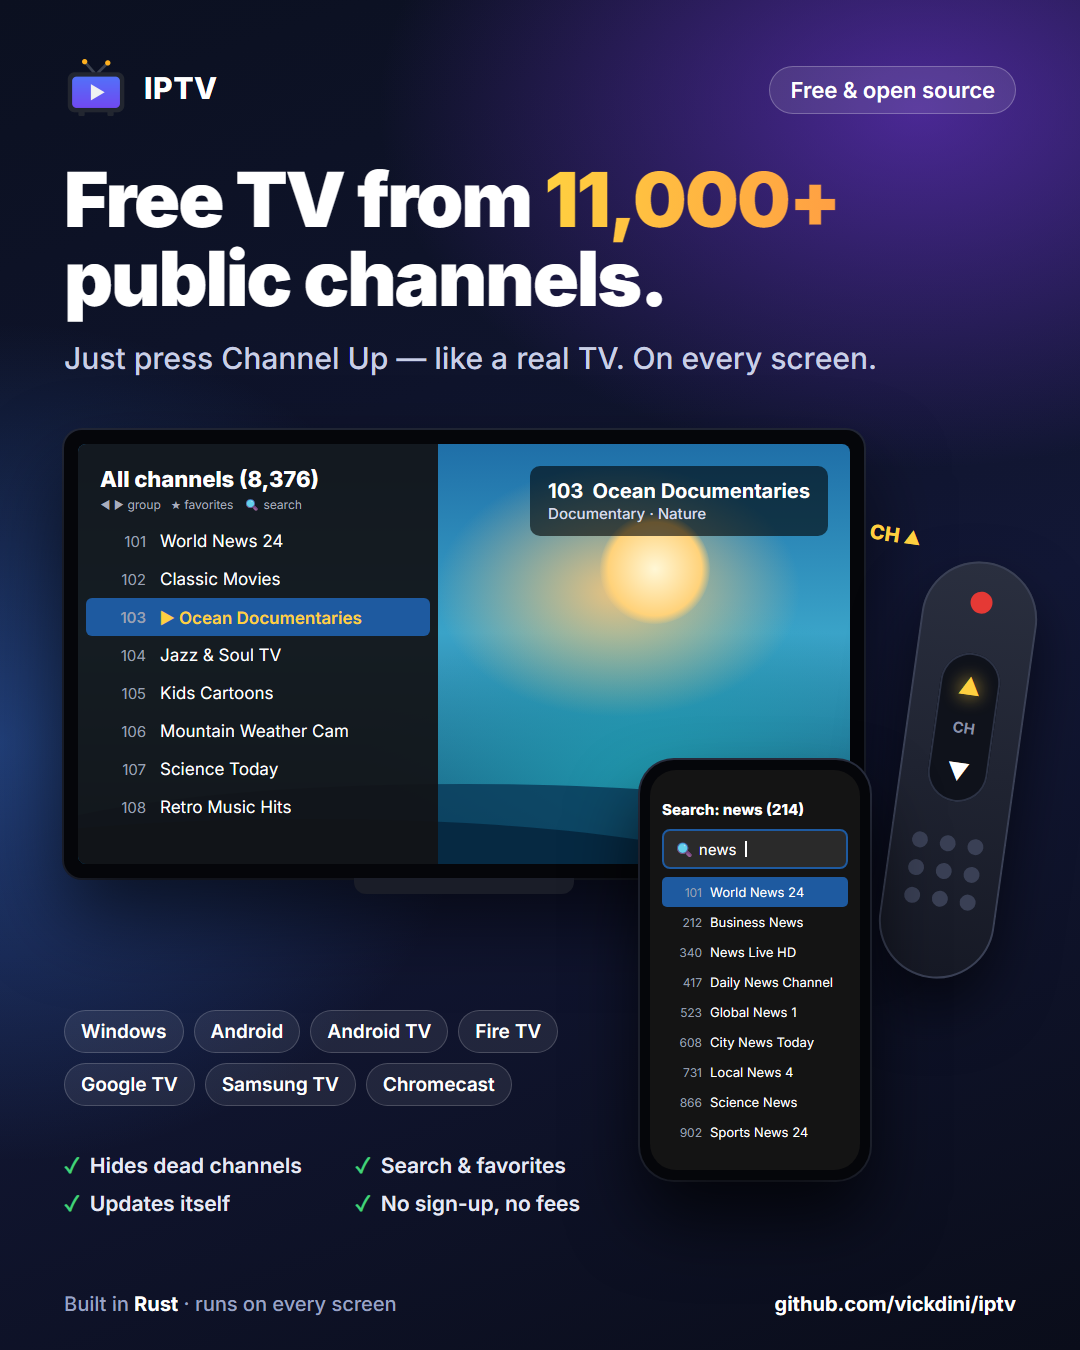
\includegraphics[width=0.52\textwidth]{../images/iptv-overview.png}\par
  \vfill
  {\large Windows \textbullet{} macOS \textbullet{} Linux \textbullet{} Android
   \textbullet{} Android TV \& Fire TV \textbullet{} Chromecast \textbullet{} Samsung TV\par}
  \vspace{0.5cm}
  {\color{dim} #2 \version{} \textbullet{} \url{https://github.com/vickdini/iptv}\par}
\end{titlepage}
\tableofcontents
\thispagestyle{fancy}}
:
%   \GuideLang   babel language (english, italian, spanish, french, ngerman, portuguese)
%   \GuideTitle  the guide's title, used on the cover, in headers and the PDF
%   \TipLabel    the word that starts a tip box ("Tip.")
% Build any of them with pdflatex, twice (for the table of contents).
\documentclass[11pt,a4paper]{article}

\usepackage[T1]{fontenc}
\usepackage[utf8]{inputenc}
% shorthands=off: no language-specific active characters (they would clash
% with tables and addresses); only hyphenation and "Contents" etc. change.
\usepackage[shorthands=off,\GuideLang]{babel}
\usepackage{lmodern}
\usepackage[scaled=0.92]{helvet}
\renewcommand{\familydefault}{\sfdefault}
\usepackage[margin=2.2cm,headheight=14pt]{geometry}
\usepackage{graphicx}
\usepackage[table]{xcolor}
\usepackage{booktabs}
\usepackage{tabularx}
\usepackage{xltabular}
\usepackage{enumitem}
\usepackage{titlesec}
\usepackage{fancyhdr}
\usepackage{pifont}
\usepackage{amssymb}
\usepackage[hidelinks]{hyperref}

\newcommand{\version}{0.12}
\definecolor{accent}{HTML}{1E6FD9}
\definecolor{dim}{HTML}{5F6673}
\definecolor{notebg}{HTML}{EEF4FC}
\definecolor{warnbg}{HTML}{FFF6E0}
\definecolor{tvred}{HTML}{D32F2F}
\definecolor{tvgreen}{HTML}{2E7D32}
\definecolor{tvyellow}{HTML}{C9A400}
\definecolor{tvblue}{HTML}{1565C0}

\hypersetup{pdftitle={IPTV -- \GuideTitle}, pdfauthor={IPTV project}}
\setlist{itemsep=2pt, topsep=4pt}
\setlength{\parindent}{0pt}
\setlength{\parskip}{6pt}
\renewcommand{\arraystretch}{1.25}

\titleformat{\section}{\Large\bfseries\color{accent}}{\thesection}{0.6em}{}
\titleformat{\subsection}{\large\bfseries}{\thesubsection}{0.6em}{}
\titlespacing*{\section}{0pt}{14pt}{6pt}
\titlespacing*{\subsection}{0pt}{10pt}{4pt}

\pagestyle{fancy}
\fancyhf{}
\fancyhead[L]{\small\color{dim}IPTV -- \GuideTitle}
\fancyhead[R]{\small\color{dim}github.com/vickdini/iptv}
\fancyfoot[C]{\small\color{dim}\thepage}
\renewcommand{\headrulewidth}{0.4pt}
\renewcommand{\sectionmark}[1]{\markboth{#1}{}}

% A key or button on a keyboard / remote.
\newcommand{\key}[1]{{\setlength{\fboxsep}{1.5pt}\fbox{\footnotesize\vphantom{Ay}#1}}}
% A coloured remote button.
\newcommand{\colorkey}[2]{\textcolor{#1}{\ding{108}}\,\textbf{#2}}
% Shaded boxes for tips and notes.
\newcommand{\tip}[1]{\par\noindent\colorbox{notebg}{\parbox{\dimexpr\linewidth-2\fboxsep}{\small\textbf{\TipLabel} #1}}\par}
\newcommand{\note}[1]{\par\noindent\colorbox{warnbg}{\parbox{\dimexpr\linewidth-2\fboxsep}{\small #1}}\par}
\newcommand{\menu}[1]{\textit{#1}}
\newcommand{\download}{\url{https://github.com/vickdini/iptv/releases/latest}}
% Key tables: \rowcolors{2}{gray!8}{white} then
% \begin{xltabular}{\linewidth}{@{}KX@{}} \keyshead{Key}{What it does} ... \bottomrule
\newcolumntype{K}{>{\raggedright\arraybackslash}p{5.4cm}}
\newcommand{\keyshead}[2]{\toprule \textbf{#1} & \textbf{#2} \\ \midrule}

% The cover: #1 subtitle, #2 "Version".
\newcommand{\cover}[2]{%
\begin{titlepage}
  \centering
  \vspace*{0.5cm}
  {\fontsize{40}{48}\selectfont\bfseries\color{accent} IPTV\par}
  \vspace{0.3cm}
  {\LARGE \GuideTitle\par}
  \vspace{0.3cm}
  {\large\color{dim} #1\par}
  \vspace{1cm}
  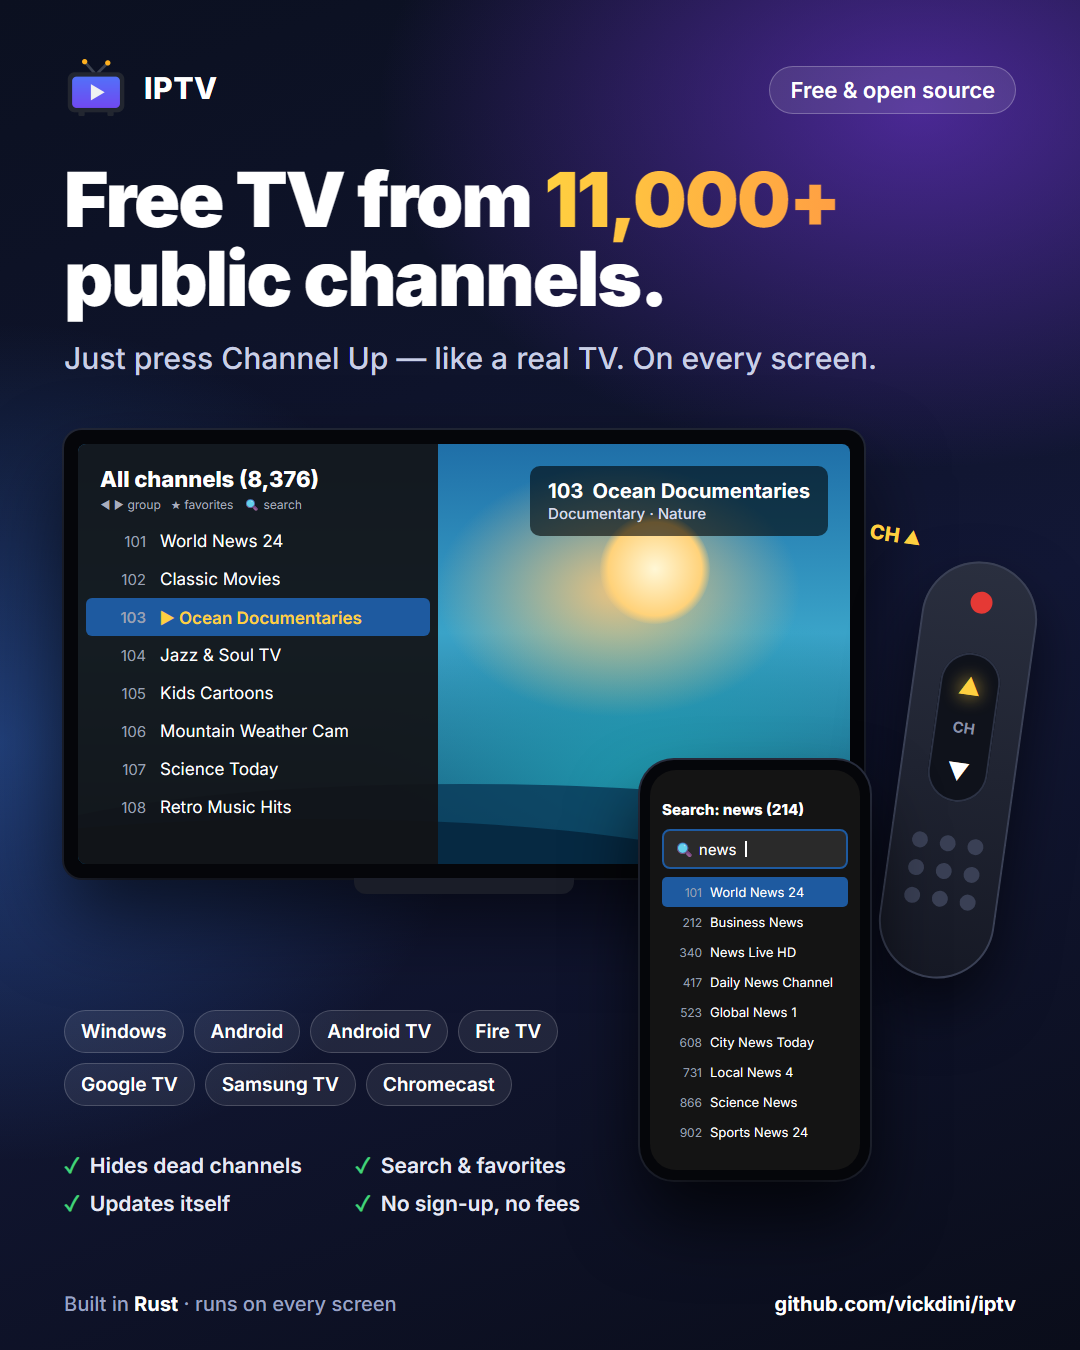
\includegraphics[width=0.52\textwidth]{../images/iptv-overview.png}\par
  \vfill
  {\large Windows \textbullet{} macOS \textbullet{} Linux \textbullet{} Android
   \textbullet{} Android TV \& Fire TV \textbullet{} Chromecast \textbullet{} Samsung TV\par}
  \vspace{0.5cm}
  {\color{dim} #2 \version{} \textbullet{} \url{https://github.com/vickdini/iptv}\par}
\end{titlepage}
\tableofcontents
\thispagestyle{fancy}}
:
%   \GuideLang   babel language (english, italian, spanish, french, ngerman, portuguese)
%   \GuideTitle  the guide's title, used on the cover, in headers and the PDF
%   \TipLabel    the word that starts a tip box ("Tip.")
% Build any of them with pdflatex, twice (for the table of contents).
\documentclass[11pt,a4paper]{article}

\usepackage[T1]{fontenc}
\usepackage[utf8]{inputenc}
% shorthands=off: no language-specific active characters (they would clash
% with tables and addresses); only hyphenation and "Contents" etc. change.
\usepackage[shorthands=off,\GuideLang]{babel}
\usepackage{lmodern}
\usepackage[scaled=0.92]{helvet}
\renewcommand{\familydefault}{\sfdefault}
\usepackage[margin=2.2cm,headheight=14pt]{geometry}
\usepackage{graphicx}
\usepackage[table]{xcolor}
\usepackage{booktabs}
\usepackage{tabularx}
\usepackage{xltabular}
\usepackage{enumitem}
\usepackage{titlesec}
\usepackage{fancyhdr}
\usepackage{pifont}
\usepackage{amssymb}
\usepackage[hidelinks]{hyperref}

\newcommand{\version}{0.12}
\definecolor{accent}{HTML}{1E6FD9}
\definecolor{dim}{HTML}{5F6673}
\definecolor{notebg}{HTML}{EEF4FC}
\definecolor{warnbg}{HTML}{FFF6E0}
\definecolor{tvred}{HTML}{D32F2F}
\definecolor{tvgreen}{HTML}{2E7D32}
\definecolor{tvyellow}{HTML}{C9A400}
\definecolor{tvblue}{HTML}{1565C0}

\hypersetup{pdftitle={IPTV -- \GuideTitle}, pdfauthor={IPTV project}}
\setlist{itemsep=2pt, topsep=4pt}
\setlength{\parindent}{0pt}
\setlength{\parskip}{6pt}
\renewcommand{\arraystretch}{1.25}

\titleformat{\section}{\Large\bfseries\color{accent}}{\thesection}{0.6em}{}
\titleformat{\subsection}{\large\bfseries}{\thesubsection}{0.6em}{}
\titlespacing*{\section}{0pt}{14pt}{6pt}
\titlespacing*{\subsection}{0pt}{10pt}{4pt}

\pagestyle{fancy}
\fancyhf{}
\fancyhead[L]{\small\color{dim}IPTV -- \GuideTitle}
\fancyhead[R]{\small\color{dim}github.com/vickdini/iptv}
\fancyfoot[C]{\small\color{dim}\thepage}
\renewcommand{\headrulewidth}{0.4pt}
\renewcommand{\sectionmark}[1]{\markboth{#1}{}}

% A key or button on a keyboard / remote.
\newcommand{\key}[1]{{\setlength{\fboxsep}{1.5pt}\fbox{\footnotesize\vphantom{Ay}#1}}}
% A coloured remote button.
\newcommand{\colorkey}[2]{\textcolor{#1}{\ding{108}}\,\textbf{#2}}
% Shaded boxes for tips and notes.
\newcommand{\tip}[1]{\par\noindent\colorbox{notebg}{\parbox{\dimexpr\linewidth-2\fboxsep}{\small\textbf{\TipLabel} #1}}\par}
\newcommand{\note}[1]{\par\noindent\colorbox{warnbg}{\parbox{\dimexpr\linewidth-2\fboxsep}{\small #1}}\par}
\newcommand{\menu}[1]{\textit{#1}}
\newcommand{\download}{\url{https://github.com/vickdini/iptv/releases/latest}}
% Key tables: \rowcolors{2}{gray!8}{white} then
% \begin{xltabular}{\linewidth}{@{}KX@{}} \keyshead{Key}{What it does} ... \bottomrule
\newcolumntype{K}{>{\raggedright\arraybackslash}p{5.4cm}}
\newcommand{\keyshead}[2]{\toprule \textbf{#1} & \textbf{#2} \\ \midrule}

% The cover: #1 subtitle, #2 "Version".
\newcommand{\cover}[2]{%
\begin{titlepage}
  \centering
  \vspace*{0.5cm}
  {\fontsize{40}{48}\selectfont\bfseries\color{accent} IPTV\par}
  \vspace{0.3cm}
  {\LARGE \GuideTitle\par}
  \vspace{0.3cm}
  {\large\color{dim} #1\par}
  \vspace{1cm}
  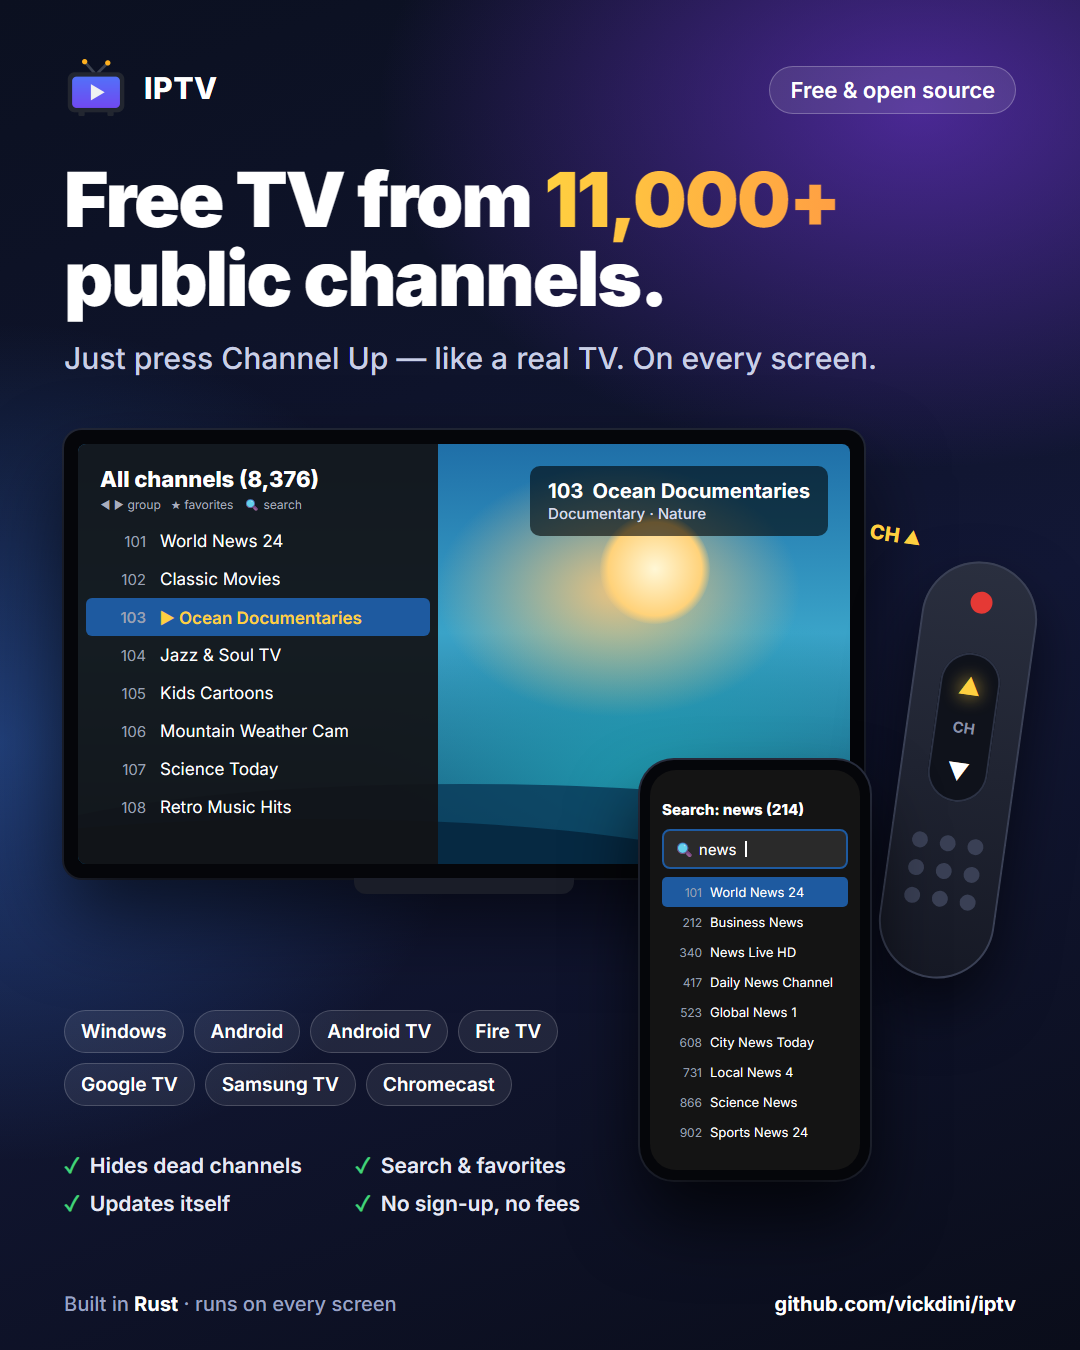
\includegraphics[width=0.52\textwidth]{../images/iptv-overview.png}\par
  \vfill
  {\large Windows \textbullet{} macOS \textbullet{} Linux \textbullet{} Android
   \textbullet{} Android TV \& Fire TV \textbullet{} Chromecast \textbullet{} Samsung TV\par}
  \vspace{0.5cm}
  {\color{dim} #2 \version{} \textbullet{} \url{https://github.com/vickdini/iptv}\par}
\end{titlepage}
\tableofcontents
\thispagestyle{fancy}}


\begin{document}
\cover{Guarda canali TV gratuiti e fai zapping come su un televisore}{Versione}

% ------------------------------------------------------------------ intro
\section{Cos'è IPTV}

IPTV riproduce i canali TV gratuiti e pubblicamente elencati raccolti dal
progetto \emph{iptv-org} (più di 10\,000) e ti permette di passare dall'uno
all'altro come su un televisore: canale su e giù, numeri dei canali,
preferiti e gruppi come Notizie, Film o Sport.

\begin{itemize}
  \item \textbf{Sempre aggiornato.} L'elenco dei canali viene aggiornato a ogni
        avvio e l'app si aggiorna da sola quando esce una nuova versione.
  \item \textbf{Solo canali che funzionano.} I canali non disponibili vengono
        nascosti automaticamente, così lo zapping non si ferma mai su uno
        schermo nero.
  \item \textbf{Trovi subito i canali.} Cerca per nome, riconosci ogni canale
        dal logo, torna ai canali visti di recente o mostra solo i paesi e le
        lingue che ti interessano.
  \item \textbf{La tua lingua.} IPTV parla italiano, inglese, spagnolo,
        francese, tedesco e portoghese, e segue la lingua del dispositivo. Sui
        canali che le trasmettono, scegli la lingua dell'audio e attiva i
        sottotitoli.
  \item \textbf{Telecomando dal telefono.} Controlla la TV o il computer dal
        browser del telefono (sezione~\ref{sec:remote}).
\end{itemize}

Ogni download contiene tutto il necessario: non c'è nient'altro da
installare. Tutti i download sono nella pagina delle versioni:

\begin{center}
  \download
\end{center}

\note{\textbf{Avvertenza.} IPTV non ospita né fornisce alcun video: carica
solo una playlist pubblica pubblicata dal progetto iptv-org. Guarda solo ciò
che puoi guardare legalmente nel tuo paese.}

% ------------------------------------------------------------------ Windows
\section{Windows}
\label{sec:windows}

\subsection{Installazione}
\begin{enumerate}
  \item Scarica \texttt{IPTV-Setup-\textless versione\textgreater.exe} dalla
        pagina delle versioni e aprilo.
  \item Se Windows mostra \menu{PC protetto da Windows}, fai clic su
        \menu{Ulteriori informazioni} e poi su \menu{Esegui comunque}.
  \item Segui il programma di installazione. Non servono diritti di
        amministratore; aggiunge un collegamento nel menu Start (e, se vuoi,
        un'icona sul desktop).
\end{enumerate}
IPTV si apre a finestra intera e inizia subito a trasmettere. Per
disinstallarlo, usa \menu{Impostazioni \textrightarrow{} App}.

\subsection{Tasti}
\label{sec:keys}
Questi tasti funzionano su tutti i computer: Windows, macOS e Linux.

\rowcolors{2}{gray!8}{white}
\begin{xltabular}{\linewidth}{@{}KX@{}}
\keyshead{Tasto}{Funzione}
\key{$\uparrow$} \key{$\downarrow$}, \key{PagSu} \key{PagGiù}, rotellina & canale successivo / precedente \\
\key{0}--\key{9}, poi attendi o \key{Invio} & vai a un numero di canale \\
\key{Backspace} & torna al canale precedente \\
\key{$\leftarrow$} \key{$\rightarrow$}, \key{m} & volume giù / su, muto \\
\key{l}, \key{Tab} o clic destro & apri / chiudi l'elenco dei canali \\
\key{/} o \key{Ctrl}+\key{F} & cerca i canali per nome \\
\key{c} & scegli paesi e lingue \\
\key{g} / \key{G} & visti di recente, poi i gruppi (Notizie, Film\ldots) \\
\key{s} / \key{S} & aggiungi o togli un preferito / zapping solo tra i preferiti \\
\key{a} / \key{t} & lingua audio successiva / sottotitoli successivi (e disattivati) \\
\key{r} & telecomando dal telefono: mostra il codice QR \\
\key{E} / \key{I} & esporta / importa i preferiti (cartella Download) \\
\key{i} & informazioni sul canale \\
\key{f}, doppio clic & schermo intero (\key{Esc} per uscire) \\
\key{p} & riquadro: un secondo canale, piccolo, nell'angolo in basso a destra \\
\key{[} / \key{]} & canale precedente / successivo del riquadro \\
\key{x}, clic sul riquadro & scambia i due canali \\
\key{Spazio} & pausa \\
\key{h}, \key{?} o \key{F1} & aiuto sullo schermo \\
\key{q} & esci \\
\bottomrule
\end{xltabular}

\subsection{L'elenco dei canali}
Premi \key{l} per aprire a sinistra un elenco scorrevole dei canali, con i
loro loghi; il video continua accanto. Scorri con la rotellina e fai clic su
un canale per guardarlo. Inizia a scrivere (o premi \key{/}) per cercare:
accenti e maiuscole non contano. \key{Esc} chiude l'elenco. Premi \key{g} per
i canali visti di recente, dal più recente.

\subsection{Paesi e lingue}
Premi \key{c}, scrivi per trovare un paese o una lingua e premi \key{Invio}
per spuntarlo; \key{Tab} passa da un elenco all'altro. Da quel momento IPTV
mostra solo i canali dei paesi spuntati o nelle lingue spuntate, finché non
azzeri la scelta (\key{Canc}, o la riga \emph{Azzera tutti i filtri}).

\subsection{Lingua dell'audio e sottotitoli}
Quando un canale offre più lingue audio o dei sottotitoli, una nota in basso
sullo schermo lo segnala. Premi \key{a} per la lingua audio successiva e
\key{t} per i sottotitoli successivi (e infine \emph{disattivati}). IPTV
ricorda la lingua e la usa su tutti gli altri canali che la offrono.

\subsection{Lingua e aggiornamenti}
IPTV usa la lingua del sistema. A ogni avvio controlla se c'è una nuova
versione; se c'è, la installa in silenzio e si riavvia da solo dopo qualche
secondo.

% ------------------------------------------------------------------ macOS
\section{macOS}

\subsection{Installazione}
\begin{enumerate}
  \item Controlla quale chip ha il tuo Mac: \menu{menu Apple
        \textrightarrow{} Informazioni su questo Mac}.
  \item Scarica l'immagine disco corrispondente dalla pagina delle versioni:
  \begin{itemize}
    \item Apple silicon (M1, M2, M3, M4\ldots):
          \texttt{IPTV-\textless versione\textgreater-macOS-arm64.dmg}
    \item Intel: \texttt{IPTV-\textless versione\textgreater-macOS-x86\_64.dmg}
  \end{itemize}
  \item Aprila e trascina \textbf{IPTV} su \textbf{Applicazioni}.
\end{enumerate}

\subsection{Primo avvio}
IPTV non è autenticato da Apple, quindi la prima volta macOS si rifiuta di
aprirlo. Serve una sola volta:
\begin{enumerate}
  \item Apri IPTV da Applicazioni. Quando macOS dice che non può essere
        aperto, fai clic su \menu{Fine}.
  \item Apri \menu{Impostazioni di Sistema \textrightarrow{} Privacy e
        sicurezza}, scorri fino a \menu{«IPTV» è stato bloccato\ldots} e fai
        clic su \menu{Apri comunque}, poi conferma.
\end{enumerate}

\subsection{Uso}
IPTV usa gli stessi tasti di Windows (sezione~\ref{sec:keys}). Nel Dock
compare come \textbf{IPTV} mentre trasmette un canale.

\tip{Tieni IPTV nella cartella Applicazioni: avviato dall'immagine disco o
dalla cartella Download, macOS lo esegue da una copia di sola lettura e non
può aggiornarsi.}

% ------------------------------------------------------------------ Linux
\section{Linux}

\subsection{Installazione}
Scarica \texttt{IPTV-\textless versione\textgreater-x86\_64.AppImage} dalla
pagina delle versioni. È un unico file che contiene tutto. Rendilo
eseguibile e avvialo:
\begin{center}
\begin{minipage}{0.8\linewidth}
\small\ttfamily chmod +x IPTV-*-x86\_64.AppImage\\
./IPTV-*-x86\_64.AppImage
\end{minipage}
\end{center}
In alternativa, in un file manager apri \menu{Proprietà \textrightarrow{}
Permessi}, spunta \menu{Consenti l'esecuzione come programma} e fai doppio
clic sul file.

Funziona sui PC a 64 bit con un Linux del 2022 o più recente (Ubuntu 22.04,
Debian 12, Fedora 36, Linux Mint 21 e successivi).

\tip{Strumenti come \emph{Gear Lever} o \emph{AppImageLauncher} aggiungono
IPTV al menu delle applicazioni. Se l'AppImage segnala che manca FUSE,
avvialo con \texttt{-{}-appimage-extract-and-run}.}

\subsection{Uso}
IPTV usa gli stessi tasti di Windows (sezione~\ref{sec:keys}). Si aggiorna
sostituendo il file AppImage, quindi tienilo in una cartella in cui puoi
scrivere (per esempio la tua cartella home).

% ------------------------------------------------------------------ Android
\section{Telefoni e tablet Android}

\subsection{Installazione}
\begin{enumerate}
  \item Sul telefono, scarica \texttt{IPTV-\textless versione\textgreater.apk}
        dalla pagina delle versioni e aprilo.
  \item Android chiede una volta di consentire l'installazione di app dal
        browser o dal file manager: consentila, poi tocca \menu{Installa}.
  \item IPTV non è su Google Play, quindi Play Protect potrebbe avvisare di
        uno sviluppatore sconosciuto: scegli \menu{Installa comunque}.
\end{enumerate}
Puoi anche installarlo con \emph{Obtainium}, che tiene aggiornate le app
direttamente dalla loro pagina delle versioni.

\subsection{Gesti}
\rowcolors{2}{gray!8}{white}
\begin{xltabular}{\linewidth}{@{}KX@{}}
\keyshead{Gesto}{Funzione}
scorri su / giù & canale successivo / precedente \\
tocca & apri / chiudi l'elenco dei canali \\
doppio tocco & torna al canale precedente \\
tocco prolungato & informazioni sul canale \\
\bottomrule
\end{xltabular}

\subsection{Due canali insieme}
Tieni il telefono o il tablet in verticale e lo schermo si divide in due, un
canale sopra l'altro. Tocca una metà per sentirla: un sottile bordo blu la
indica, e l'elenco dei canali e il telecomando dal telefono agiscono su di
essa. Scorri su o giù su una metà per cambiarne il canale. Rimetti il
dispositivo in orizzontale per un solo canale.

\subsection{Picture-in-picture}
Esci dall'app mentre guardi (tasto Home, o scorri verso l'alto dal fondo):
il canale continua in una piccola finestra sopra le altre app, con i pulsanti
per cambiare canale. Tocca la finestra per tornare a IPTV, o trascinala via
per chiuderla. Richiede Android 8 o successivo.

\subsection{L'elenco dei canali}
Tocca lo schermo per aprirlo. Tocca un canale per guardarlo, tienilo premuto
per aggiungerlo ai preferiti o toglierlo. I pulsanti in alto:
\begin{itemize}
  \item Casella di \textbf{ricerca}: scrivi parte del nome di un canale.
  \item Frecce $\blacktriangleleft$\,$\blacktriangleright$: gruppo
        precedente / successivo.
  \item \textbf{Orologio}: i canali visti di recente.
  \item $\bigstar$: solo preferiti. Tienilo premuto per salvare i preferiti in
        un file o aggiungerli da un file.
  \item \textbf{Globo}: scegli paesi e lingue.
  \item \textbf{Sottotitoli} (solo sui canali che offrono una scelta): lingua
        dell'audio e sottotitoli.
  \item \textbf{Telecomando dal telefono}: controlla IPTV da un altro
        telefono (sezione~\ref{sec:remote}).
  \item \textbf{Trasmetti}: riproduci su un Chromecast
        (sezione~\ref{sec:chromecast}).
  \item \textbf{Esci}: chiude IPTV (e interrompe la trasmissione).
\end{itemize}

\subsection{Lingua e aggiornamenti}
IPTV usa la lingua del telefono. All'avvio controlla se c'è una nuova
versione. La prima volta Android chiede di consentire a IPTV di installare
app; in seguito gli aggiornamenti si installano con al massimo una conferma.

% ------------------------------------------------------------------ Android TV
\section{Android TV, Google TV e Fire TV}

La stessa app funziona sui dispositivi TV e si usa con il telecomando. Gli
store per TV non la offrono, quindi si installa una volta con l'app gratuita
\emph{Downloader}:

\begin{itemize}
  \item \textbf{Fire TV / Fire TV Stick:} installa \emph{Downloader}
        dall'Amazon Appstore. Poi apri \menu{Impostazioni \textrightarrow{} La
        mia Fire TV \textrightarrow{} Opzioni sviluppatore \textrightarrow{}
        Installa app sconosciute} e attiva Downloader.
  \item \textbf{Google TV, Chromecast con Google TV, Android TV:} installa
        \emph{Downloader} dal Play Store e consentilo in
        \menu{Impostazioni \textrightarrow{} App \textrightarrow{} Sicurezza e
        limitazioni \textrightarrow{} Origini sconosciute}.
\end{itemize}
In Downloader, inserisci
\begin{center}
  \download
\end{center}
poi scarica \texttt{IPTV-\textless versione\textgreater.apk} e installalo.
IPTV comparirà tra le app della TV.

\subsection{Telecomando}
\rowcolors{2}{gray!8}{white}
\begin{xltabular}{\linewidth}{@{}KX@{}}
\keyshead{Tasto}{Funzione}
Su / Giù, Canale +/$-$, Avanti / Indietro veloce & canale successivo / precedente \\
OK, Play/Pausa, Menu & apri / chiudi l'elenco dei canali \\
Sinistra / Destra & visti di recente, poi i gruppi \\
0--9 (se il telecomando li ha) & vai a un numero di canale \\
Indietro & chiudi l'elenco \\
Info & informazioni sul canale \\
Tasti Audio / CC (se presenti) & lingua audio / sottotitoli successivi \\
\bottomrule
\end{xltabular}

Nell'elenco dei canali, premi Su sul primo canale per raggiungere la casella
di ricerca. I pulsanti in alto nell'elenco scelgono paesi e lingue, audio e
sottotitoli, e aprono il telecomando dal telefono.

\tip{La maggior parte di questi telecomandi non ha tasti numerici: il
telecomando dal telefono (sezione~\ref{sec:remote}) è il modo più rapido per
scegliere un canale.}

% ------------------------------------------------------------------ Chromecast
\section{Chromecast}
\label{sec:chromecast}

I Chromecast più vecchi (la chiavetta semplice senza telecomando) non possono
installare app. Trasmetti su di essi dall'app Android:
\begin{enumerate}
  \item Assicurati che il telefono e il Chromecast siano sulla stessa rete
        Wi-Fi.
  \item Apri l'elenco dei canali in IPTV, tocca il pulsante
        \textbf{Trasmetti} e scegli il tuo Chromecast.
  \item Fai zapping sul telefono come al solito: la TV segue.
\end{enumerate}
Alcuni canali non si possono trasmettere perché i loro server non lo
consentono; IPTV li salta automaticamente.

% ------------------------------------------------------------------ Samsung
\section{Smart TV Samsung}

IPTV funziona sulle TV Samsung dal 2019 in poi. Samsung permette di
installare app che non sono nel suo store solo da un computer, con la TV in
\emph{modalità sviluppatore}. La configurazione si fa una volta sola, da un PC
Windows sulla stessa rete Wi-Fi della TV.

\subsection{Installazione}
\begin{enumerate}
  \item Sul PC, installa gli strumenti a riga di comando di \emph{Tizen
        Studio} da \url{https://developer.tizen.org}. Nel suo Package Manager,
        installa \emph{Samsung Certificate Extension} e \emph{TV Extensions
        Tools} (scheda \menu{Extension SDK}).
  \item Sulla TV, apri \menu{App} e digita \key{1}\key{2}\key{3}\key{4}\key{5}
        con il telecomando. Attiva la \menu{modalità sviluppatore}, inserisci
        l'indirizzo IP del PC e riavvia la TV.
  \item Scarica \texttt{IPTV-Samsung-TV-\textless versione\textgreater.zip}
        dalla pagina delle versioni ed estrailo.
  \item Trova l'indirizzo IP della TV (\menu{Impostazioni \textrightarrow{}
        Generali \textrightarrow{} Rete \textrightarrow{} Stato della rete}) ed
        esegui, nella cartella estratta:
\begin{center}
\begin{minipage}{0.92\linewidth}
\small\ttfamily powershell -ExecutionPolicy Bypass -File install-on-tv.ps1 -TvIp 192.168.1.4
\end{minipage}
\end{center}
        La prima volta spiega come creare il certificato Samsung gratuito
        (accedendo con un account Samsung). Eseguilo di nuovo dopo: installa
        IPTV, che poi compare tra le App della TV.
\end{enumerate}
Da quel momento IPTV si aggiorna da solo: non serve ripetere la
configurazione per le nuove versioni. Usa la lingua della TV.

\subsection{Telecomando}
\rowcolors{2}{gray!8}{white}
\begin{xltabular}{\linewidth}{@{}KX@{}}
\keyshead{Tasto}{Funzione}
Su / Giù, CH + / CH $-$ & canale successivo / precedente \\
0--9 & vai a un numero di canale \\
OK & elenco dei canali (nell'elenco: guarda il canale selezionato) \\
Sinistra / Destra & visti di recente, poi i gruppi \\
PRE-CH & torna al canale precedente \\
INFO & informazioni sul canale \\
\colorkey{tvred}{Rosso} & aggiungi o togli un preferito \\
\colorkey{tvgreen}{Verde} & solo preferiti \\
\colorkey{tvyellow}{Giallo} & menu lingua audio e sottotitoli \\
\colorkey{tvyellow}{Giallo} nell'elenco & scegli paesi e lingue \\
\colorkey{tvblue}{Blu} & cerca i canali per nome \\
Indietro & chiudi l'elenco, o esci da IPTV \\
\bottomrule
\end{xltabular}

\note{Il telecomando dal telefono (sezione~\ref{sec:remote}) non è ancora
disponibile sulle TV Samsung. L'app gratuita \emph{SmartThings} funziona come
telecomando dal telefono per i tasti principali.}

% ------------------------------------------------------------------ remote
\section{Telecomando dal telefono}
\label{sec:remote}

Controlla IPTV dal telefono, Android o iPhone, senza installare nulla. Puoi
sfogliare e cercare tutti i canali e toccarne uno per guardarlo; il
telecomando ha anche i preferiti, i canali visti di recente, canale su / giù,
volume, lingua dell'audio e sottotitoli. Funziona con IPTV sul computer e su
Android TV, Google TV e Fire TV, e parla la lingua del tuo telefono.

\begin{enumerate}
  \item Sul computer premi \key{r}. Su Android TV, Google TV o Fire TV, apri
        l'elenco dei canali e scegli il pulsante \textbf{telecomando dal
        telefono}. Compare un codice QR.
  \item Inquadralo con la fotocamera del telefono. Il telefono deve essere
        sulla stessa rete Wi-Fi. Senza fotocamera, apri nel browser del
        telefono l'indirizzo mostrato sullo schermo e inserisci il PIN.
  \item Il telecomando si apre nel browser del telefono. Aggiungilo alla
        schermata Home o ai segnalibri: da quel momento si collega da solo
        ogni volta che IPTV è acceso.
\end{enumerate}

Per spostare i preferiti su un'altra TV o un altro computer, usa
\textbf{Salva sul telefono} in fondo alla pagina del telecomando, poi
\textbf{Aggiungi da un file} nel telecomando dell'altro dispositivo. I
preferiti vengono aggiunti, mai rimossi. Sul computer puoi anche premere
\key{E} (salva nella cartella Download) e \key{I} (aggiungi da lì); su
telefoni e tablet Android, tieni premuto il pulsante $\bigstar$.

\note{La prima volta, Windows (e macOS, se il firewall è attivo) chiede se
IPTV può usare la rete: consentilo sulle reti \textbf{private}, altrimenti i
telefoni non riescono a collegarsi. Solo i telefoni che conoscono il PIN
possono controllare IPTV.}

% ------------------------------------------------------------------ help
\section{Risoluzione dei problemi}

\begin{description}[style=nextline, leftmargin=0pt, itemsep=6pt]
  \item[Un canale non parte.] Molti canali gratuiti vanno offline o
        funzionano solo in alcuni paesi. IPTV li nasconde e passa oltre da
        solo; basta cambiare canale.
  \item[L'elenco sembra più corto di prima.] Controlla se sono scelti dei
        paesi o delle lingue (\key{c} sul computer, il pulsante del globo su
        Android, \colorkey{tvyellow}{Giallo} nell'elenco sulle TV Samsung) e
        azzerali.
  \item[Il telecomando dal telefono non si collega.] Verifica che il telefono
        sia sulla stessa rete Wi-Fi (non sui dati mobili) e che il firewall
        del computer consenta IPTV sulle reti private.
  \item[I sottotitoli sono elencati ma non compare nulla.] Alcuni canali
        annunciano sottotitoli che in realtà non inviano. IPTV funziona
        correttamente.
  \item[IPTV è nella lingua sbagliata.] Segue la lingua del dispositivo (sul
        computer, quella del sistema). I nomi dei canali, dei gruppi e dei
        paesi provengono dalla playlist e sono sempre in inglese.
  \item[Altro?] Segnalalo su \url{https://github.com/vickdini/iptv/issues}.
\end{description}

\vfill
{\small\color{dim} IPTV è software libero, rilasciato con la GNU General
Public License, versione 3 o successiva. Il codice sorgente è su
\url{https://github.com/vickdini/iptv}.\par}

\end{document}
